\subsection {(Dis)Charge Circuitry}

This subsection will explain the circuit used to (dis)charge the DUT and the circuit used to measure the current through the DUT.

The basic purpose of this section is to measure the charge/discharge curves of the DUT by stepping the input voltage and then measuring the current through the device over time.

\begin{figure}[ht!]
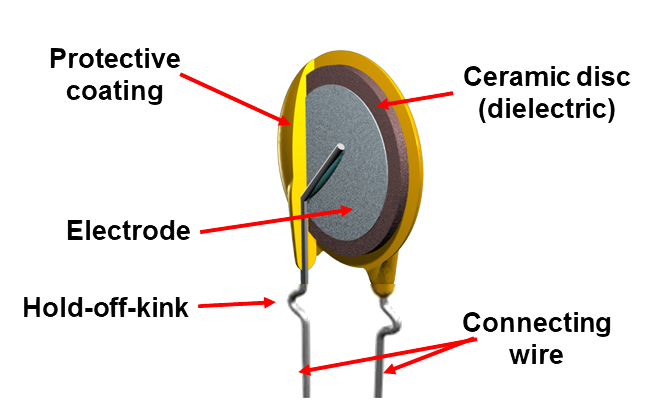
\includegraphics[keepaspectratio=true,scale=.5]{./figures/testImage.png}
\centering
\caption{(Dis)(Charge) Block Diagram}
\label{fig:cdlBlock}
\end{figure}


The block diagram depicted in Figure: \ref{cdlBlock} shows how this section will function. There are three basic modes:

Charging:
In this mode, the supply is set to the desired voltage and then stepped into the circuit with a relay. The input voltage sees a known resistor in series with the DUT to a virtual ground. The DUT will charge up to the input voltage according to its time constant. The virtual ground is made up of a transimpedance amplifier. It has the advantage of being able to measure on the low side of the DUT.

Discharging:
With the Charging side disconnected, a relay can connect the discharging circuitry to ground through a series resistor. The current measurement circuitry performs the same function, but with the opposite polarity measurement.

Leakage:
Once the DUT is charged to its full voltage, the steady state current can be measured over a much larger time period.


